\section{Experimental Evaluation}
\label{par:Discussion}

\subsection{Visualizer}
\label{sec:Vizualizer}
In order to make the debugging more easier we developed a visualization program, ``CurveReconDriver''. CurveReconDriver is a multi-platform program that runs on Windows, Linux and Mac OS X. With this program we can draw points or let the program generate a given number of random points. The feature set of CurveReconDrive also includes the importing and exporting of test cases, from which to generate curves. This program is very useful to detect errors in our different implementations, because it helps to visually see the wrong decisions our algorithms made.\\
We ran a number of test-cases to test our algorithms. The test-cases were generated using our visualization program, which has the ability to draw points. This enabled us to easily generate test-cases and test them using the same program. Since the visualization program automatically draws the algorithm's output, errors are easily spotted. (Take, for example, intersections on a closed curve test-case). The program also has a random point generation option.\\
We ran the experiments on a HP Compaq 8510w Laptop with the following specifications:\\
2,4 GHz Intel Core 2 Duo processor T7700\\
2 GB memory.\\

\begin{figure}[!h!b!t]
\begin{center}
  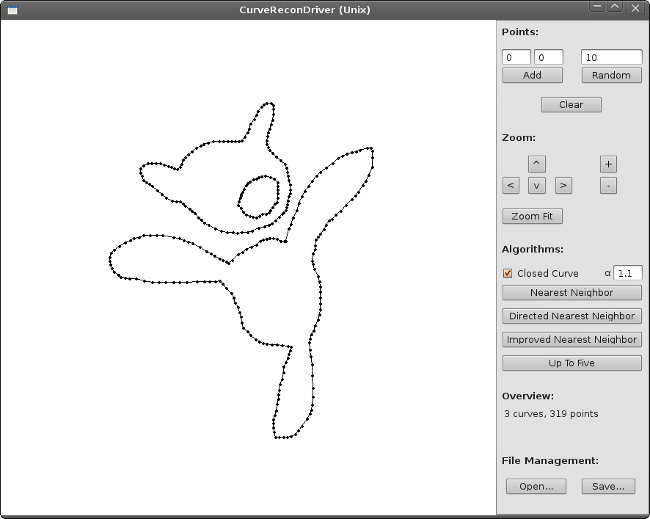
\includegraphics[scale=0.4]{Discussion/newdebugprogram.png}
  \label{fig:gui}\\
  Figure 3.1: GUI of visualization
\end{center}
\end{figure}

\subsection{Nearest Neighbor}
  \label{sub:nn_test_results}
    \textbf{Running time}\\
    We first tested our algorithm on randomly generated points (solely for determining the running time of the algorithm).\\
    The results are given in the Table 3.1 and Figure 3.2.

      \begin{center}
        \begin{tabular}{|p{2.5cm}|p{2.5cm}|}
            \hline
            Points & Seconds\\
            \hline
            \hline
            500 & 0.015\\
            \hline
            1000 & 0.016\\
            \hline
            1500 & 0.047\\
            \hline
            2000 & 0.078\\
            \hline
            5000 & 0.442\\
            \hline
            10000 & 1.669\\
            \hline
            15000 & 4.087\\
            \hline
            20000 & 6.755\\
            \hline
            30000 & 16.552\\
            \hline
            40000 & 27.878\\
            \hline
            50000 & 47,768\\
            \hline
            60000 & 66.16\\
            \hline
            80000 & 108.358\\
            \hline
            100000 & 202.239\\
            \hline
        \end{tabular}
        \label{tab:nn_runningtime}\\
        Table 3.1: A table of our results on testing \textit{NearestNeighbor}
    \end{center}

    \begin{center}
      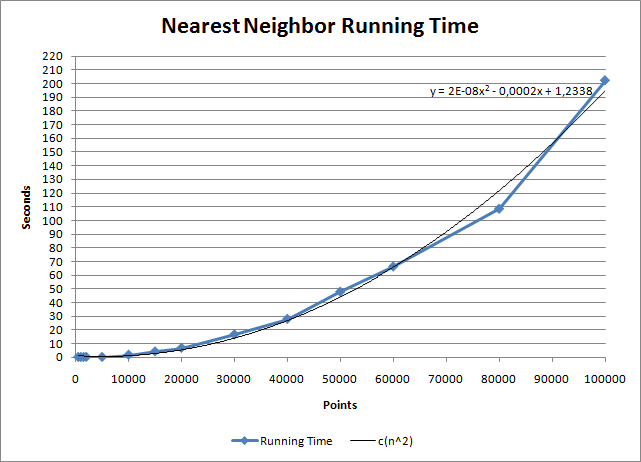
\includegraphics[scale = 0.5]{1NearestNeighbor/nnRuntimegraph.png}\\
      Figure 3.2: Graph of \textit{NearestNeighbor}'s Running Time
      \label{fig:nn_runningtime}
    \end{center}
    This graph tells us that our analysis of the running time (\ref{sub:nearest_neighbor}) is correct: when the number of input points are doubled, the running time is quadrupled $(2^2)$, when they are tripled, the running time is multiplied by roughly $3^2$, etc.\\
    Along with the resulting graph of the test, we introduced a trend line (which is a $n^2$ function fitted to our test results) to show the running time is indeed $O(n^2)$.\\
    So, we can conclude that in practice this algorithm is $O(n^2)$ too.\\ \\ \\
    \textbf{Correct output}\\
    We analyzed a few test-cases that failed giving the correct output.\\
    We give suggestions as to what caused this behavior, and supply possible solutions below.\\

    \noindent An example of a test-case in which \textit{NearestNeighbor} fails is the Heart with 200 points. As you can see in Figure 3.3 there are two places the curve starts zigzagging between points.
    This problem occurs because the correct point in this case is not the nearest neighbor of the previous one. This could be corrected by taking the curve's current direction into account. This way, we could prevent the curve from jumping around.\\
    \noindent Another failed test-case is the Spiral with 91 points (Figure 3.4). Here, we experience the same problem as in the first case, that is, going in the wrong direction because the nearest point is not the correct successor. We also see another problem caused by this: when the spiral is nearly complete, the algorithm picks the points, which haven't been processed yet. In this case those points reside at the other side of the spiral.\\
    \noindent The third test-case is the ``8'' with 364 points (Figure 3.5). The problem here is that is does not intersect. Nearest Neighbor does not make sure there is at least one intersection. So, another thing we should take into consideration is that we need to check for intersections. \\
    \noindent The fourth and last test-case we discuss is the Flat with 178 points. This problem could also be solved by keeping track of the curve's current direction, so that it will not end up zigzagging again (marked in Figure 3.6).\\\\
        \begin{center}
        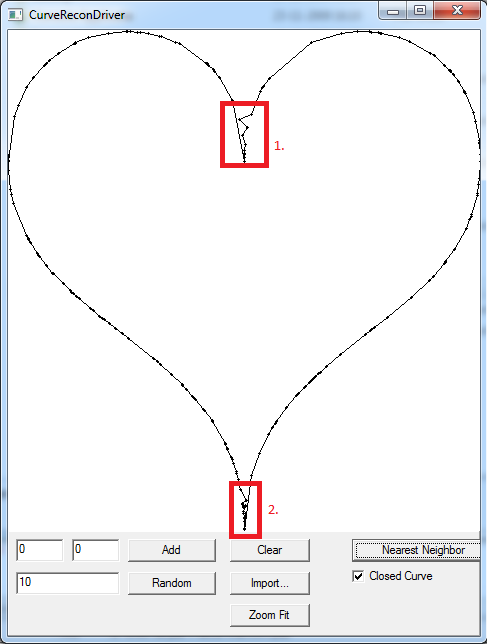
\includegraphics[scale = 0.45]{1NearestNeighbor/nnHeartgraph.png}\\
        \label{fig:nn_incorrectheart}
        Figure 3.3: Incorrect heart
        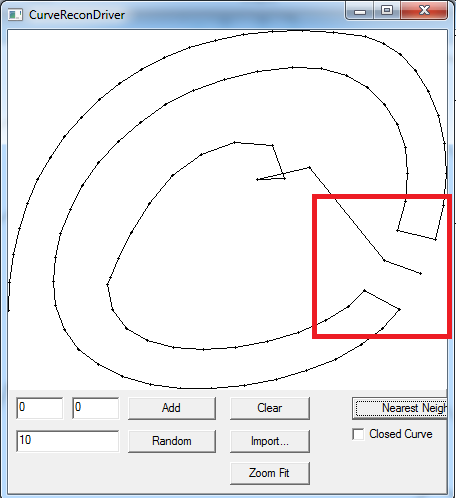
\includegraphics[scale = 0.5]{1NearestNeighbor/nnSpiralgraph.png}\\
        \label{fig:nn_incorrectspiral}
        Figure 3.4: Incorrect spiral
        {\ }\\[1.0cm]
        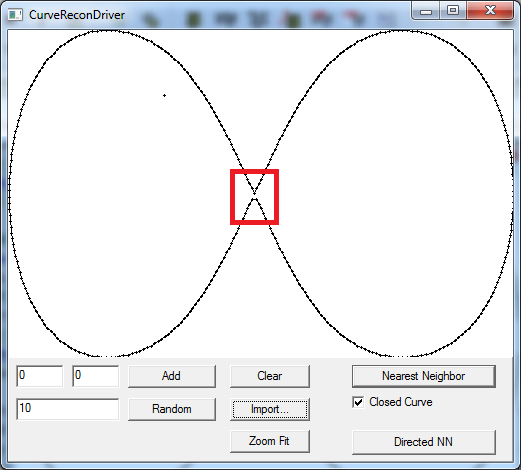
\includegraphics[scale = 0.5]{1NearestNeighbor/nnEightgraph.png}\\
        \label{fig:nn_incorrecteight}
        Figure 3.5: Incorrect eight
        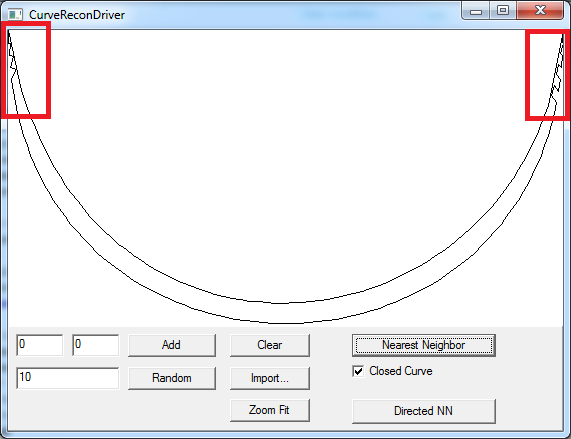
\includegraphics[scale = 0.5]{1NearestNeighbor/nnFlatgraph.png}\\
        \label{fig:nn_incorrectflat}
        Figure 3.6: Incorrect flat
        \end{center}
    \textbf{Conclusion}\\
    From all these test results we can conclude there are a number of things that need improving. We could, for example (as mentioned before), look at the curve's direction, which would fix the zigzagging. We should also check for intersections when the input requires it.

    \subsection{Directed Nearest Neighbor}
  \label{sub:dnn_test_results}
    \textbf{Running time}\\
        To determine the running time of the Directed Nearest Neighbor algorithm, we first tested our algorithm on randomly generated points.\\
        We ran the experiments on a HP Compaq 8510w Laptop with the following specifications:\\
        2,4 GHz Intel Core 2 Duo processor T7700\\
        2 GB memory.
        The results are given in Table 3.2 and Figure 3.7. The constant used by the algorithm was set at $1.5$, meaning the range for \textit{FindPointsInRange} is the length of the last-drawn line multiplied by $1.5$.

        \begin{center}
          \begin{tabular}{|p{2.5cm}|p{2.5cm}|}
              \hline
              Points & Seconds\\
              \hline
              \hline
              500 & 0.015\\
              \hline
              1000 & 0.047\\
              \hline
              1500 & 0.078\\
              \hline
              2000 & 0.14\\
              \hline
              5000 & 0.624\\
              \hline
              10000 & 2.246\\
              \hline
              15000 & 5.414\\
              \hline
              20000 & 9.407\\
              \hline
              30000 & 20.936\\
              \hline
              40000 & 45.864\\
              \hline
              50000 & 63.367\\
              \hline
              60000 & 93.335\\
              \hline
              80000 & 183.772\\
              \hline
          \end{tabular}
          \label{tab:dnn_runningtime}\\
          Table 3.2: Results of testing \textit{DirectedNearestNeighbor}
        \end{center}

        \begin{center}
        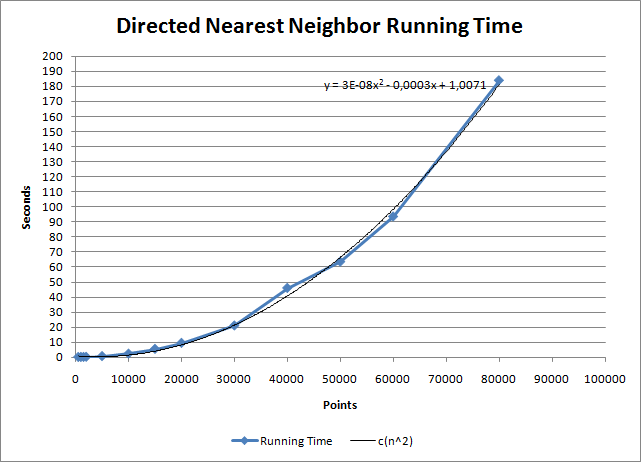
\includegraphics[scale = 0.5]{2DirectedNearestNeighbor/dnnRuntimeGraph.png}\\
        Figure 3.7: Graph of \textit{DirectedNearestNeighbor}'s Running Time
        \label{fig:dnn_runnningtime}
        \end{center}

        \noindent When comparing the above running times to the ones from Nearest Neighbor, we observe this algorithm is indeed a little slower as we have shown in the running time analysis (~\ref{sub:directed_nearest_neighbor}). However, when we introduce a trend line that derives a $n^2$ function from the results, we see that the algorithm is still $O(n^2)$.\\\\
        \textbf{Correct Output}\\
        After testing some of the test-cases, we noticed some of the previous algorithm's problems were now solved. The Flat test-case with 178 points was constructed correctly with the DirectedNearestNeighbor.

        \begin{center}
        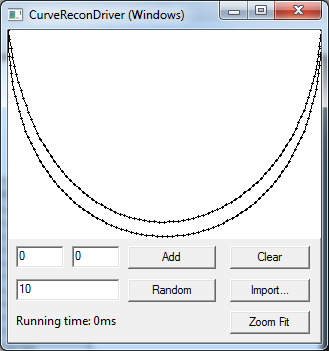
\includegraphics[scale = 0.6]{2DirectedNearestNeighbor/dnnFlatgraph.png}\\
        \label{fig:ddn correctflat}
        Figure 3.8: Correct Flat
        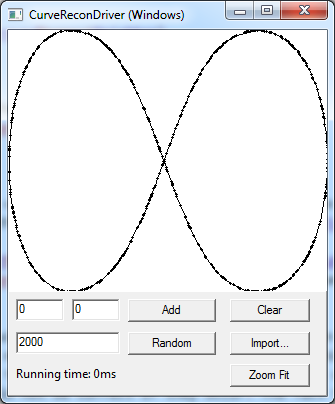
\includegraphics[scale = 0.6]{2DirectedNearestNeighbor/dnnEightGraph.png}\\
        \label{fig:ddn correctflat}
        Figure 3.9: Correct ``8''
        \end{center}
        But we also noticed test-cases still going wrong, this is due to that the algorithm still does not check for intersections when they are needed or not, another possibility is a non-optimal choice of the constant for determine the range. A clear example of this is the Spiral test-case. When we ran this with the above stated constant, we saw that because there were two points really close to each other (see red square in Figure 3.10), it does not choose the point after it correctly. This is because the next line to be drawn is much longer than $1.5$ times the small line between the previous two points.\\
        \noindent Another thing we noticed was that the problem of lines going right through the graph still existed (and maybe even got worse, see Figure 3.11). This is because, now that the algorithm is pickier, more points are left at the end. Since the algorithm wants to connect all points, it picks the ones left at the end.
        A solution for this could be checking for unused points at the end, and then try to insert these point in the correct place.
        \begin{center}
        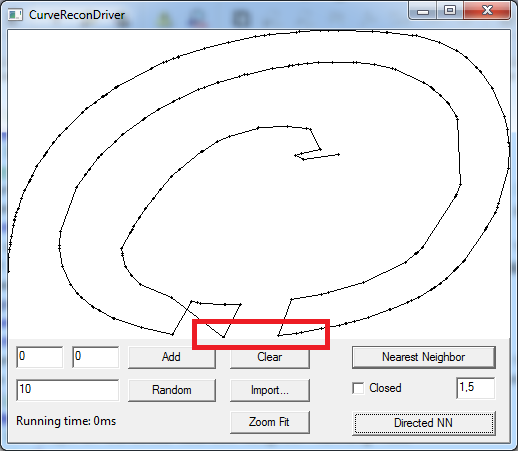
\includegraphics[scale = 0.5]{2DirectedNearestNeighbor/dnnSpiralgraph.png}\\
        \label{fig:dnn_incorrectspiral}
        Figure 3.10: Incorrect Spiral
        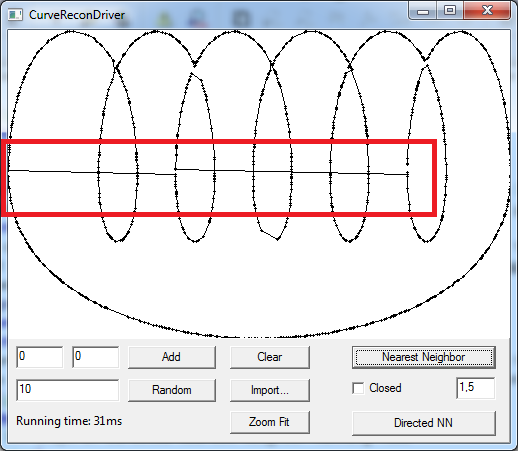
\includegraphics[scale = 0.5]{2DirectedNearestNeighbor/dnnSpringgraph.png}\\
        \label{fig:dnn_incorrectspring}
        Figure 3.11 Incorrect Spring
       \end{center}
        \textbf{Conclusion}\\
        When we look at several incorrect test-cases, we see that we need a better way of picking the range for Find-Points-In-Range. Also, we need to check for unused or incorrectly inserted points at the end. This is needed to make sure the points are inserted correctly and not just connected to each other at the end, messing up the curve. Another thing we could improve on is to look more carefully at the curve's direction, instead of just looking at angles to points in a certain range. Another improvement we should consider is to check for intersections at the end of reconstruction.
\newpage
  \subsection{Improved Nearest Neighbor}
  \label{sub:inn_test_results}
    \textbf{Running time}\\
        The results for our \textit{ImprovedNearestNeighbor} are given in Table 3.3 and Figure 3.12.

        \begin{center}
          \begin{tabular}{|p{2.5cm}|p{2.5cm}|}
              \hline
              Points & Seconds\\
              \hline
              \hline
              500 & 0.016\\
              \hline
              1000 & 0.032\\
              \hline
              1500 & 0.078\\
              \hline
              2000 & 0.156\\
              \hline
              5000 & 1.591\\
              \hline
              10000 & 6.755\\
              \hline
              15000 & 10.935\\
              \hline
              20000 & 17.659\\
              \hline
              30000 & 36.738\\
              \hline
              40000 & 59.202\\
              \hline
              50000 & 107.360\\
              \hline
              60000 & 154.582\\
              \hline
              80000 & 240.034\\
              \hline
          \end{tabular}
          \label{tab:inn_runningtime}\\
          Table 3.3: Results of testing \textit{ImprovedNearestNeighbor}
        \end{center}

          \begin{center}
            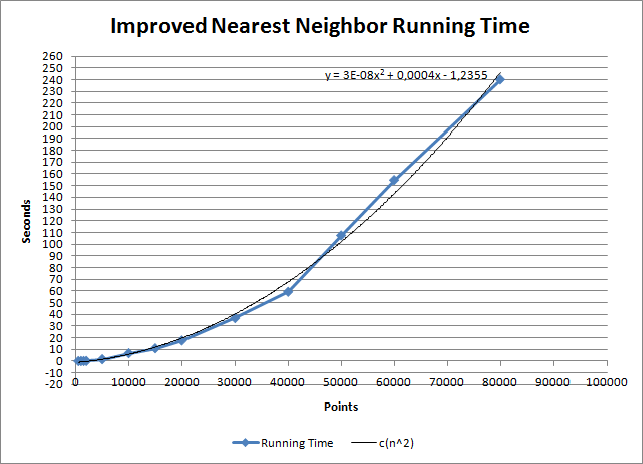
\includegraphics[scale = 0.5]{3ImprovedNearestNeighbor/innRuntimeGraph.png}\\
            Figure 3.12: Graph of \textit{ImprovedNearestNeighbor}'s Running Time
            \label{fig:inn_runnningtime}
          \end{center}

      \noindent The results of the running time are what we expected, again it looks like the algorithm is $O(n^2)$, especially when we introduce the $n^2$ trend line. It may not be that obvious as it was the case with \textit{NearestNeighbor} and \textit{DirectedNearestNeighbor} but we still can conclude using the graph that \textit{ImprovedNearestNeighbor} is $O(n^2)$.
      If we compare the algorithm to \textit{NearestNeighbor} and \textit{DirectedNearestNeighbor}, we see that is slower than \textit{NearestNeighbor}, which is obvious of course since it uses \textit{NearestNeighbor} with an extra function, and faster than \textit{DirectedNearestNeighbor}.\\\\
    \textbf{Correct output}\\
    There were a couple of things that went better with \textit{ImprovedNearestNeighbor} than with \textit{NearestNeighbor}. For example the heart of 128 points (See figure 3.14), which went completely right. Another thing that works much better in Improved Nearest is the following closed curve, when we draw a normal circle with one point at the outside \textit{NearestNeighbor} would fail but the new \textit{ImprovedNearestNeighbor} does not. This is because of the new functionality to insert points at the end, which checks for multiple things which would not be correct if they occur. The fact that the reconstruction of this type of curve has improved is good, since a similar type of curve can be found in several other test-cases we ran.
    See Figure 3.13 to see an example.\\

          \begin{center}
            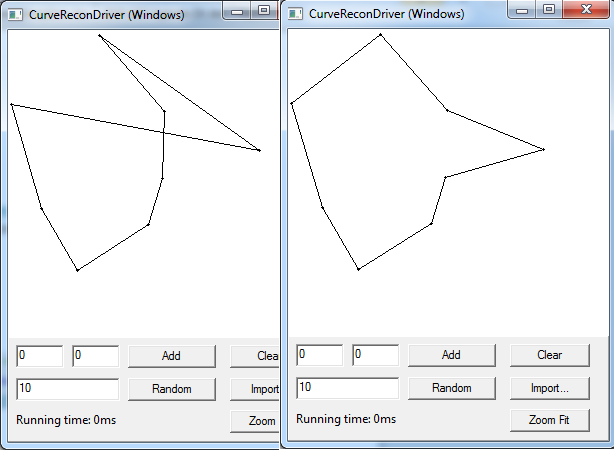
\includegraphics[scale = 0.5]{3ImprovedNearestNeighbor/innPointCirkel.png}\\
            Figure 3.13: Left: Nearest Neighbor Algorithm. Right: Improved Nearest Neighbor Algorithm
            \label{fig:inn_pointcircle}
          \end{center}
\newpage
   \noindent For example one of the test cases which contains this problem; the Heart with 128 points:\\
          \begin{center}
            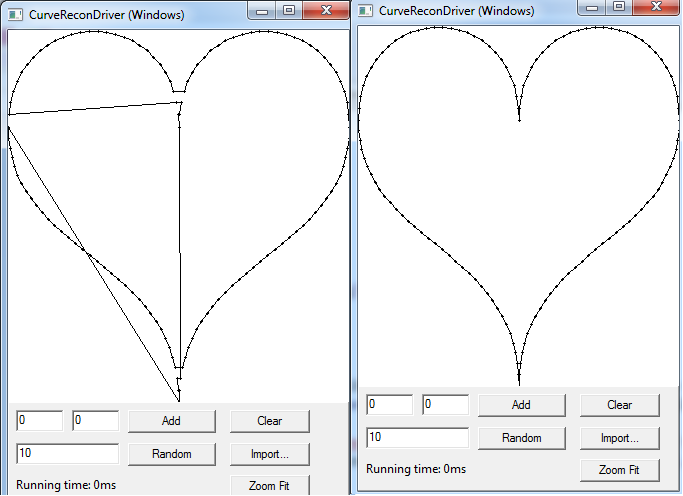
\includegraphics[scale = 0.4]{3ImprovedNearestNeighbor/innHeart.png}\\
            Figure 3.14: Left: Nearest Neighbor Algorithm. Right: Improved Nearest Neighbor Algorithm
            \label{fig:inn_pointcircle}
          \end{center}

    \noindent A test case that still went wrong is the spiral: \\
          \begin{center}
            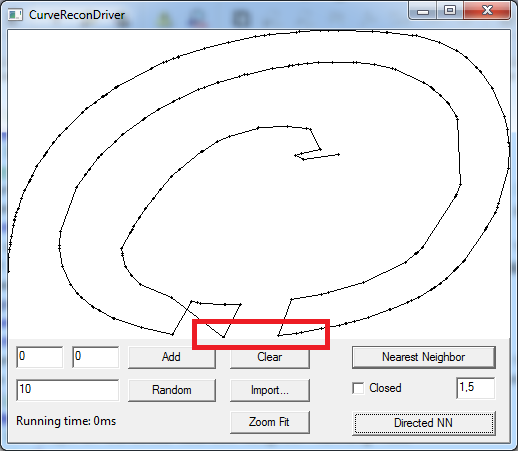
\includegraphics[scale = 0.6]{3ImprovedNearestNeighbor/innSpiral.png}\\
            Figure 3.15: Incorrect Spiral
            \label{fig:inn_pointcircle}
          \end{center}

  \noindent This test case results in the same incorrect reconstruction as with the Nearest Neighbor algorithm. So in this test case the function that inserts lost points at the end didn't have any effect. A suggestion to improve this result would be to add the technic of the Direct Nearest Neighbor to this algorithm. This could result in a much better result.

  \noindent Another test case that went wrong is the Flat with 88 points:\\

            \begin{center}
            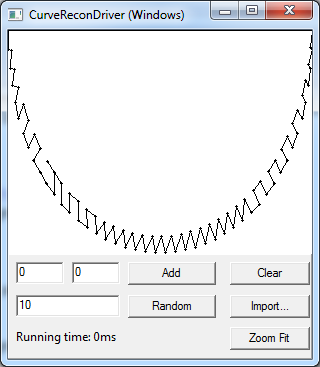
\includegraphics[scale = 0.7]{3ImprovedNearestNeighbor/innFlat.png}\\
            Figure 3.16: Incorrect Flat
            \label{fig:inn_pointcircle}
          \end{center}

  \noindent In this test case we notice some zigzagging, although this is a pretty hard test case since there are only 88 points, the same solution as mentioned above could provide a better reconstruction. Because this test case could probably benefit a lot by checking in which direction the curve is going.\\\\
   \textbf{Conclusion}\\
   We can conclude from the above experiments that Improved Nearest Neighbor really improves a number of problems we first had with the standard Nearest Neighbor algorithm. Especially the function that inserts lost points at the end really provides better results. But still there are a number of test cases that went wrong, to make this number of failing test cases smaller, a combination of the Improved and Directed Nearest Neighbor could maybe be a solution. This could, for example, result in a better reconstruction of the Spiral test case. Another thing that could probably make the reconstructions better is a check for intersections. Since a number of test cases contained a number of intersections which shouldn't be there. For example see the Spiral test case.
   These two suggestions would probably make the Improved Nearest Neighbor even better.
\newpage
    \subsection{Up To Five Sort}
  \label{sub:utfs_test_results}
    \textbf{Running time}\\
    After using the same method as before we got the following results:
        \begin{center}
          \begin{tabular}{|p{2.5cm}|p{2.5cm}|}
              \hline
              Points & Seconds\\
              \hline
              \hline
              500 & 0.015\\
              \hline
              1000 & 5.032\\
              \hline
              1500 & 7.644\\
              \hline
              2000 & 9.812\\
              \hline
              5000 & 24.805\\
              \hline
              10000 & 56.691\\
              \hline
              15000 & 77.330\\
              \hline
              20000 & 105.347\\
              \hline
              30000 & 163.100\\
              \hline
              40000 & 217.278\\
              \hline
              50000 & 281.118\\
              \hline
          \end{tabular}
          \label{tab:utfs_runningtime}\\
          Table 3.4: Results of testing \textit{UpToFiveSort}
        \end{center}

          \begin{center}
            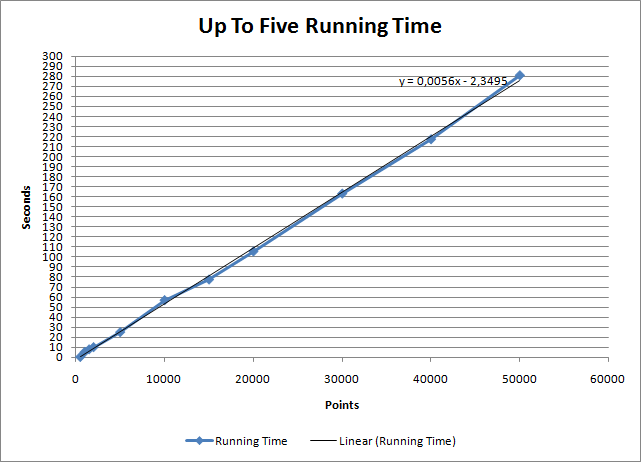
\includegraphics[scale = 0.5]{4UpToFiveSort/utfsRuntimeGraph.png}\\
            Figure 3.17: Graph of \textit{UpToFiveSort}'s Running Time
            \label{fig:utfs runningtime}
          \end{center}

      \noindent If we look at the graph of the running time we see that the algorithm look linear. But if we take in account that the running time determined in section~\ref{sub:up_to_five_sort} is $O(n^3)$ it would be unlikely that the algorithm is $O(n)$. Although the proof of the running time is determined for the worst case this is still awkward. It could of course be that the running time algorithm is really slow getting the form of a $O(n^3)$ function and the tested number of points are a very small part of this. This small part would then look like a linear function. This means that we can conclude that for most cases, in which we use this algorithm, \textit{Up To Five Sort} will have the linear running time $O(n)$.\\\\\\
    \textbf{Correct output}\\
    Since the algorithm uses much of the \textit{Nearest Neighbor} algorithm most incorrect results have similar problems as the \textit{Nearest Neighbor} algorithm.
    Most test cases with an even distance, for example the face with 134 points, or with many points, for example the house with 1000 points, went perfect.

    \begin{center}
        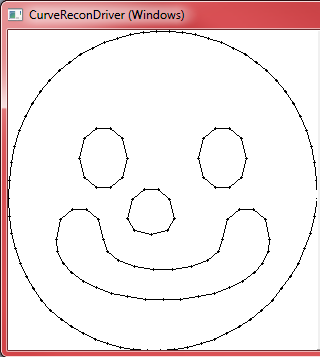
\includegraphics[scale = 0.5]{4UpToFiveSort/utfsFace.png}\\
        \label{fig:utfs_correctface}
        Figure 3.18: Correct Face
        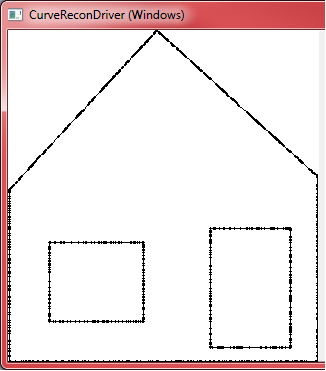
\includegraphics[scale = 0.5]{4UpToFiveSort/utfsHouse1000.png}
        \label{fig:utfs_correcthouse}\\
        Figure 3.19: Correct House of 1000 Points
    \end{center}

    But the algorithm seems to often give a incorrect solution with test cases that don't have much points.
    As an example we took the house with 200 points and 500 points.\\
    \begin{center}
        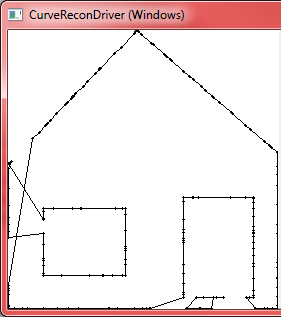
\includegraphics[scale = 0.6]{4UpToFiveSort/utfsHouse200.png}\\
        \label{fig:utfs_incorrecthouse200}
        Figure 3.20: Incorrect House of 200 Points
        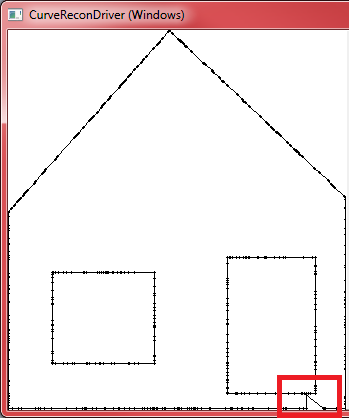
\includegraphics[scale = 0.5]{4UpToFiveSort/utfsHouse500.png}
        \label{fig:utfs_incorrecthouse500}\\
        Figure 3.21: Incorrect House of 500 Points
    \end{center}
    The first test case does not do quite well, the one of 500 points does much better except at the marked (red square in figure) section. A solution to both these problems could be checking for the direction in which the curve should go. The correctness of the reconstruction of the house with 200 points should increase although it is still difficult to determine the range in which you look for the direction the curve should go too, since there are several curves. The house with 500 points would probably be totally correct.\\
    Another test case we will be looking at is the plus test case with 120 points.

          \begin{center}
            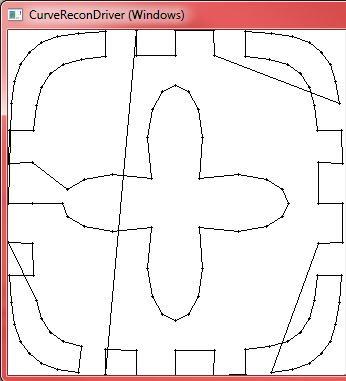
\includegraphics[scale = 0.7]{4UpToFiveSort/utfsPlus128.png}\\
            Figure 3.22: Incorrect Plus
            \label{fig:utfs incorrect plus}
          \end{center}
    We see similar problems as with the above mentioned test cases but also intersections which of course should not occur. A solution to this new problem would be some way to remove the intersections afterwards just like in the \textit{Improved Nearest Neighbor} algorithm.\\ \\ \\
   \textbf{Conclusion}\\
   From the above results we can conclude that the algorithm does give good results for most test cases although there are a couple of things that could be improved. For example taking some techniques we used in \textit{Directed Nearest Neighbor} and \textit{Improved Nearest Neighbor}, like checking the direction in which the curve is going. But these techniques are probably more difficult to insert because there are multiple curves. Since it would be much more difficult to determine the range in which you search for the next point.
